\chapter{Projeto de filtro passa-baixa butterworth de segunda ordem}
\label{apend:1}
Para o projeto do filtro, foi considerada uma frequência de corte de 15 Hz e um o período de amostragem de 0,01 segundos. Através da função \textit{butter} do MATLAB, foi realizado o cálculo dos polos do filtro, com os polos foi obtida a função de transferência no domínio da frequência por meio da função \textit{tf}. Tendo em vista que o filtro será usado em um controlador digital, a função de transferência foi convertida para o tempo discreto por meio da função \textit{c2d} para o período de amostragem de 0,01 segundos. O resultado obtido é apresentado a seguir:

\begin{equation}
    H(z) = \frac{0,1311z^2-0,2596z+0,1285}{z^2-2.007z+1,008}
    \label{transformada_filtro}
\end{equation}

Por meio da transformada Z inversa, torna-se possível obter a equação para implementação no microcontrolador, sendo y o sinal e $y_f$ o sinal filtrado para um instante de tempo k.

\begin{equation}
    y[k]= 0,7478y_f[k-1] -0,2722y_f[k-2] +0,1311y[k] +0,2622y[k-1]+0.1311y[k-2]
    \label{filtro}
\end{equation}

Com o projeto do filtro pronto, a figura a seguir mostra a comparação do sinal do \textit{encoder} do motor antes e depois do filtro.

\begin{figure}[H]
    \centering
    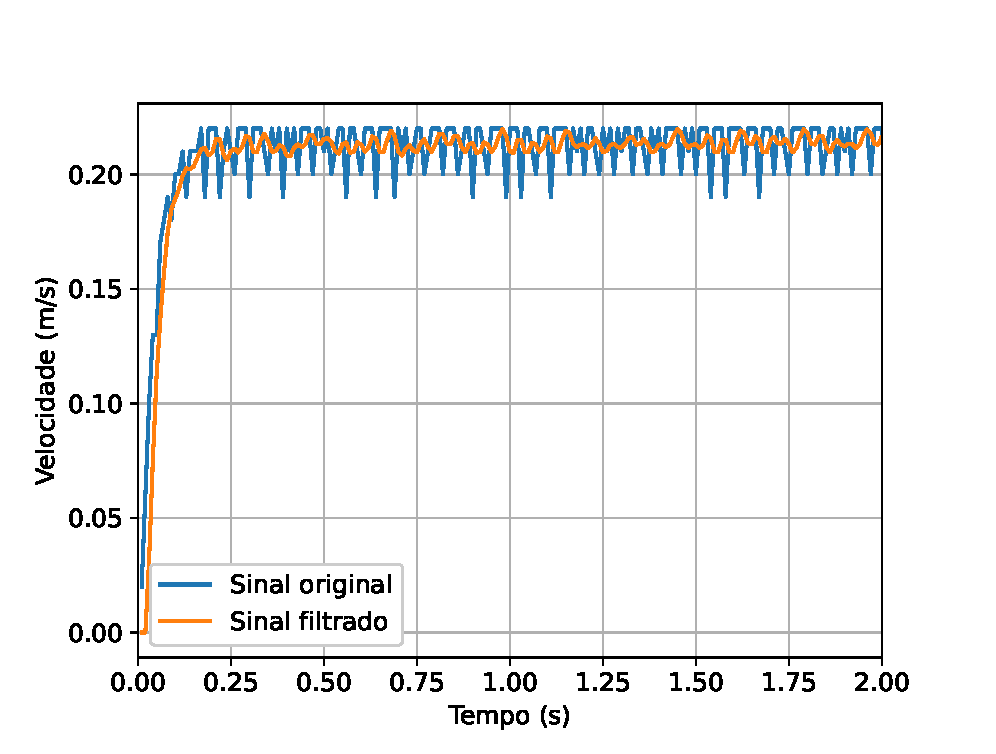
\includegraphics[width=0.8\linewidth]{figuras/filtro_12V.eps}
    \caption[Comparação do sinal do \textit{encoder} antes e depois do filtro]{Comparação do sinal do \textit{encoder} antes e depois do filtro.}
    \label{fig:resp_filtr}
\end{figure}

Pode-se observar que ocorre uma diminuição considerável do ruído na leitura do sinal, mas mesmo assim não é gerado um atraso significativo na leitura do sensor. Sendo assim, considera-se aceitável o projeto de filtro para o trabalho em questão.